\section{Durchführung und Aufbau}
\label{sec:Durchführung}
Der verwendete Versuchsaufbau besteht aus einem geschlossenen Kreislauf aus Schläuchen dreier unterschiedlicher bekannter Durchmesser, welche an einer regelbaren Zentrifugalpumpe angeschlossen sind. Diese sind mit einem Gemisch aus Wasser, Glycerin und Glaskugeln gefüllt. Auf die Schläuche wird ein Prisma wie in Abbildung \ref{fig:Doppler} zu sehen ist gesetzt um einen reproduzierbaren Dopplerwinkel $\theta$ zu garantieren.

\begin{figure}
  \centering
  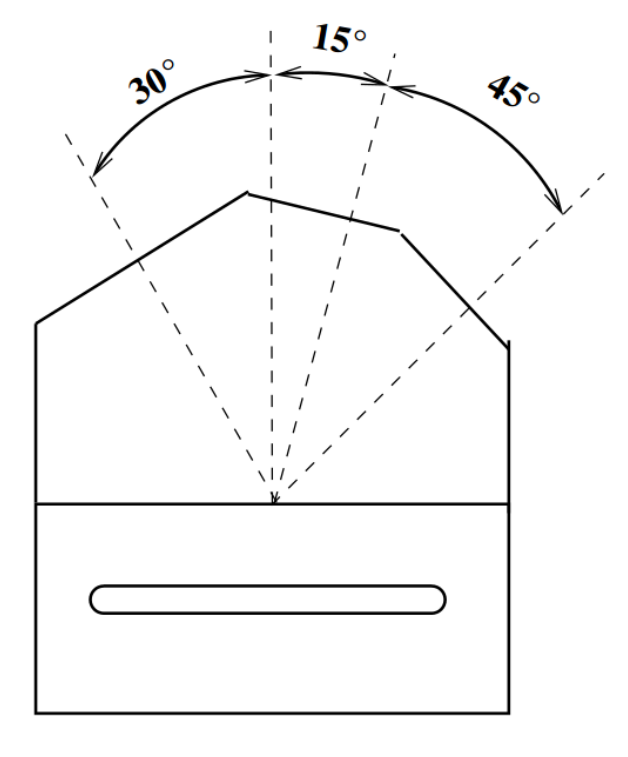
\includegraphics[height=5cm]{picture/Winkel.png}
  \caption{Winkel der Ultraschallsonde auf dem Prisma zur Berechnung des Dopllerwinkels. \cite[3]{sample}}
  \label{fig:Doppler}
\end{figure}

Auf das Prisma wird die Ultraschallsonde gehalten und die Frequenzen, sowie Eindringtiefen dem Ultraschall-Doppler-Generator bzw. dem Computer welcher zur Visualisierung dient, entnommen. An allen Kontaktstellen wird eine viskose Flüssigkeit zur besseren Leitfähigkeit draufgeschmiert.	\\
Für alle drei Schlauchdurchmesser und Dopplerwinkel wird für 5 unterschiedliche Strömungsgeschwindigkeiten die Frequenzverschiebungen gemessen. Anschließend wird bei dem Schlauch mit 1 cm Durchmesser die Eindringtiefe bei einem Prismenwinkel von 15° variiert und die Intensität der empfangenen Strahlung so wie die Frequenz gemessen. Dabei sind alle Eindringtiefen einmal abzutasten und die Messwerte zu notieren.
\newpage
